\documentclass{article}
\usepackage[dvipsnames]{xcolor}

\usepackage{tikz}
\usepackage{wrapfig}
\usepackage{bm}
\renewcommand{\baselinestretch}{1.5}


\begin{document}
\title{Chad Allen Zhao gets the hottest girl in the grade}
\author{Ramesh Balaji, Duc Nguyen, Allen Zhao}
\date{June 11, 2021}
\maketitle
Allen Zhao and Tacko Fall go on a fast break with 20 seconds left on the game clock. 
Allen must pass it directly to Fall given that Allen is accelerating at ($0.5t^2+3)\frac{ft}{sec^2}$
with an initial velocity of $14 \frac{ft}{sec}$ and an initial position of 7 ft from the half-court and Fall is accelerating at ($0.6t^2+3t) \frac{ft}{sec^2}$
with an initial velocity of $18 \frac{ft}{sec}$ and an initial position of $16 ft$ from the half-court. Allen throws the ball at 
$51 \frac{ft}{sec}$. Violet, watching the crowd has already calculated the answer to 
her challenge to Allen: to find $\frac{d\theta}{dt}$ when he throws the basketball at his
initial position. Now, Allen must do the same. 

\begin{center}
    \begin{tikzpicture}[scale=0.43]
        \draw[fill=red!10] (23,1) -- (18,1) arc[start angle=180, end angle=158.629,radius=5cm] -- (23,1);
        %\draw[fill=red!20] (23,1) -- (15,1) arc[start angle=180, end angle=158.629,radius=8cm] -- (23,1);
        %\draw[fill=blue!20] (23,1) -- (17.25,1) arc[start angle=180, end angle=167.735,radius=5.75cm] -- (23,1);
        \draw[->, >=stealth, thick] (0,-6) -- (0, 6);
        \draw[->, >=stealth, thick][dotted] (0, 6) -- (0, 10);
        \draw[->, >=stealth, thick] (23, -6) -- (23,1);
        \draw[dotted, thick]
            (0,6) -- (23,1);
        \draw[dotted, thick]
            (0,1) -- (23,1);
        \draw[dotted, thick]
            (23,1) -- (0,10);
        \draw
            (23,1) node[anchor=west] {\textbf{7 ft}};
        \draw
            (0,6) node[anchor=east] {\textbf{16 ft}};
        \draw
            (0,10) node[anchor=east] {\bm{$y_{2}(t)$}};
        \draw
            (18,1.75) node[anchor=west][scale=1.5] {\textbf{$\theta$}};
        \draw 
            (0,12) node[anchor=south] {\textbf{Tacko Fall}};
        \draw 
            (23,3) node[anchor=south] {\textbf{Allen Zhao}};
    \end{tikzpicture}
\end{center}

\begin{center}
    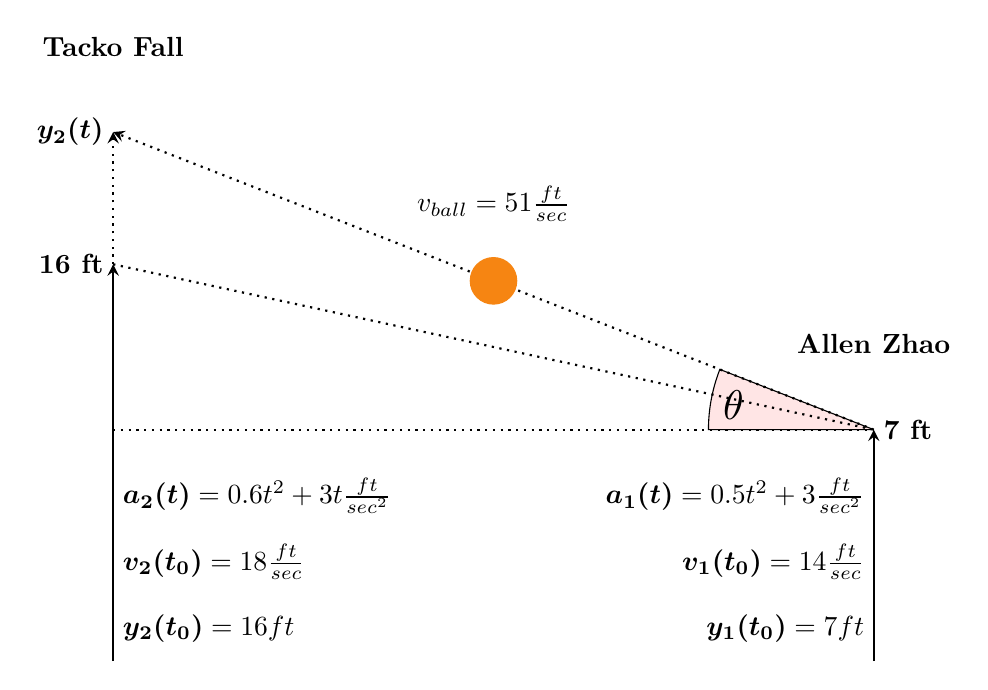
\begin{tikzpicture}[scale=0.42]
        \draw[fill=red!10] (23,1) -- (18,1) arc[start angle=180, end angle=158.629,radius=5cm] -- (23,1);
        %\draw[fill=red!20] (23,1) -- (15,1) arc[start angle=180, end angle=158.629,radius=8cm] -- (23,1);
        %\draw[fill=blue!20] (23,1) -- (17.25,1) arc[start angle=180, end angle=167.735,radius=5.75cm] -- (23,1);
        \draw[->, >=stealth, thick] (0,-6) -- (0, 6);
        \draw[->, >=stealth, thick][dotted] (0, 6) -- (0, 10);
        \draw[->, >=stealth, thick] (23, -6) -- (23,1);
        \draw[dotted, thick]
            (0,6) -- (23,1);
        \draw[dotted, thick]
            (0,1) -- (23,1);
        \draw[->, >=stealth, dotted, thick]
            (23,1) -- (0,10);
        \draw
            (23,1) node[anchor=west] {\textbf{7 ft}};

        \draw
            (0,6) node[anchor=east] {\textbf{16 ft}};
        \draw
            (0,10) node[anchor=east] {\bm{$y_{2}(t)$}};
        \draw
            (18,1.75) node[anchor=west][scale=1.5] {\textbf{$\theta$}};
        \draw 
            (0,12) node[anchor=south] {\textbf{Tacko Fall}};
        \draw 
            (23,3) node[anchor=south] {\textbf{Allen Zhao}};
        \draw
            (0,-1) node[anchor=west] {$\bm{a_{2}(t)} = 0.6t^2+3t \frac{ft}{sec^2}$};
        \draw
            (0,-3) node[anchor=west] {$\bm{v_{2}(t_{0})} = 18 \frac{ft}{sec}$};
        \draw
            (0,-5) node[anchor=west] {$\bm{y_{2}(t_{0})} = 16 ft$};
        \draw
            (23, -1) node[anchor=east] {$\bm{a_{1}(t)} = 0.5t^2 + 3 \frac{ft}{sec^2}$};
            \draw
            (23, -3) node[anchor=east] {$\bm{v_{1}(t_0)} = 14 \frac{ft}{sec}$};
        \draw 
            (23, -5) node[anchor=east] {$\bm{y_{1}(t_0)} = 7 ft$};
        \draw
            (11.5, 7) node[anchor=south] {$v_{ball} = 51 \frac{ft}{sec}$};
        \filldraw[color=BurntOrange] 
            (11.5, 5.5) circle (20pt);
    \end{tikzpicture}\par
\end{center}
    
    


\end{document}